% =====================================================================
% chapters/03_methodology.tex
% Chapter 3 — Methodology
% Project: Vision-Based Running Technique Classification from In-the-Wild
%          Internet Videos using Markerless Pose Estimation and Deep Learning
%
% Required preamble packages (declare in main.tex):
%   \usepackage{booktabs}  \usepackage{array}  \usepackage{tabularx}
%   \usepackage{graphicx}  \usepackage{amsmath}
%   \usepackage{algorithm}  \usepackage{algpseudocode}
%
% This chapter describes methods only. No empirical results appear here.
% Citation keys are drawn from references.bib and the verified project
% literature papers. Method/contribution sentences carry no citation.
% =====================================================================

\chapter{Methodology}
\label{ch:methodology}

This chapter describes the proposed framework for classifying running technique
from in-the-wild video. It follows the pipeline end to end: pose estimation,
landmark filtering and normalisation, motion-signal extraction, cycle detection,
eight-phase sampling, the two cycle representations, the classification models,
the cycle- and video-level prediction scheme, and threshold selection. No
results are reported; the experimental outcomes appear in
Chapter~\ref{ch:results}.

% ---------------------------------------------------------------------
\section{Overview of the Proposed Framework}
\label{sec:method-overview}

The framework transforms a raw video into a correct/false technique prediction
through the stages shown in Figure~\ref{fig:method_pipeline}: markerless pose
estimation, landmark filtering, motion-signal extraction, running-cycle
detection, eight-phase sampling, construction of a pose-based or image-based
representation, deep-learning classification, and evaluation. A deliberate
design principle is to keep the cycle-detection stage interchangeable so that a
manual (handmade) segmentation, a rule-based autocorrelation detector, and a
learned boundary detector can be compared under an otherwise identical pipeline,
isolating the effect of cycle source on performance.

\begin{figure}[htbp]
\centering
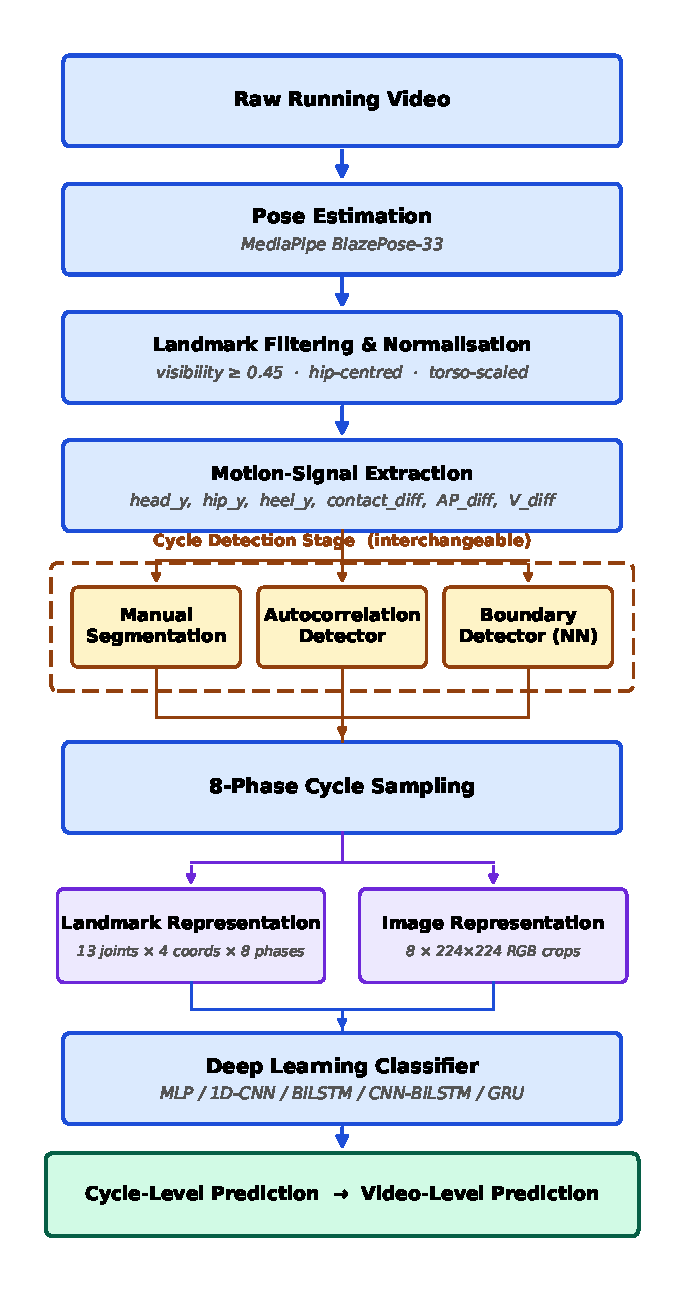
\includegraphics[width=\textwidth,height=0.75\textheight,keepaspectratio]{figures_new/fig31_pipeline}
\caption{Overall framework for vision-based running technique classification
from in-the-wild videos. Starting from a raw running video, the pipeline
applies markerless pose estimation, filters and normalises the resulting
landmarks, extracts one-dimensional motion signals, and detects running cycles
via one of three interchangeable detectors (manual, autocorrelation-based, or
learned boundary detector). Each accepted cycle is resampled into eight phases
and encoded as either a landmark sequence or a set of image crops, which are
then classified by a deep-learning model. Cycle-level predictions are
aggregated into a final video-level decision.}
\label{fig:method_pipeline}
\end{figure}


% ---------------------------------------------------------------------
\section{Dataset Construction and Splitting Protocol}
\label{sec:method-dataset}

The dataset consists of single-runner clips labelled as correct or false
technique. Because a single video yields multiple running cycles, the
\emph{splitting protocol} is critical: the data are split \emph{by video
identifier}, so that all cycles extracted from a given video are confined to a
single partition (train, validation, or test). This prevents \emph{leakage} of
video-specific information --- if cycles from one video appeared in both training
and test sets, the model could recognise the video rather than the technique,
inflating the apparent accuracy. The split is fixed once
and reused unchanged across every experiment so that all pipelines are evaluated
on the same videos. The resulting per-split counts are reported in
Chapter~\ref{ch:results}.

% ---------------------------------------------------------------------
\section{Markerless Pose Estimation}
\label{sec:method-pose}

Each frame is processed by a markerless pose estimator that returns a fixed set
of body landmarks with image coordinates and a per-landmark \emph{visibility}
(confidence) value \cite{lugaresi2019mediapipe, bazarevsky2020blazepose}. The
visibility value is retained throughout the pipeline: it is used both to filter
unreliable detections (Section~\ref{sec:method-filter}) and, in later analysis,
as a measurable proxy for input quality. A reduced set of \emph{selected
landmarks} relevant to running technique --- nose, shoulders, hips, knees,
ankles, heels, and foot indices --- is used as the basis of the pose
representation, since the discriminative information for running form is
concentrated in the trunk orientation and the lower limbs
(Chapter~\ref{ch:literature-review}). The lower-limb landmarks (ankles, heels,
toes) are the most diagnostic but also the most prone to noise and occlusion,
which motivates the filtering and normalisation described next.
Figure~\ref{fig:pose_estimation} shows an example of the estimator output on a
running frame.

\begin{figure}[htbp]
\centering
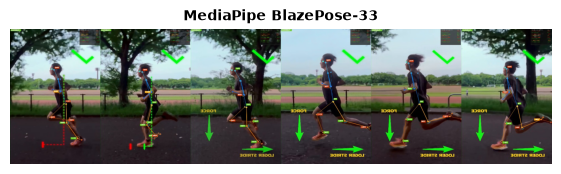
\includegraphics[width=0.60\textwidth]{figures_new/fig33_pose_estimation}
\caption{MediaPipe BlazePose-33 applied to a sample running frame. The model
produces 33 body landmarks with per-landmark visibility scores. A subset of
13 landmarks relevant to running form --- nose, hips, knees, ankles, heels,
and foot indices --- is selected for all downstream processing.}
\label{fig:pose_estimation}
\end{figure}

% ---------------------------------------------------------------------
\section{Landmark Filtering and Normalization}
\label{sec:method-filter}

Raw landmark trajectories are filtered before use. Detections whose visibility
falls below a threshold are treated as unreliable and discarded or interpolated,
and the resulting per-joint trajectories are temporally smoothed to suppress
high-frequency jitter introduced by frame-to-frame estimation noise.
Visibility-based screening is applied with particular care to the nose and heel
landmarks, which serve as quality indicators for the head and foot regions
respectively.

Landmarks are then \emph{normalised} so that the representation is invariant to
the runner's position and apparent scale in the frame. Coordinates are expressed
relative to a body-centred reference and scaled by a body-size measure (for
example a torso-span normalisation), removing dependence on where the runner
appears in the image and how far they are from the camera. This normalisation is
essential for in-the-wild video, where framing, zoom, and runner position vary
arbitrarily between clips. Figure~\ref{fig:landmark_normalization} illustrates
the effect on the vertical trajectories of the nose, hip, and heel landmarks.

\begin{figure}[htbp]
\centering
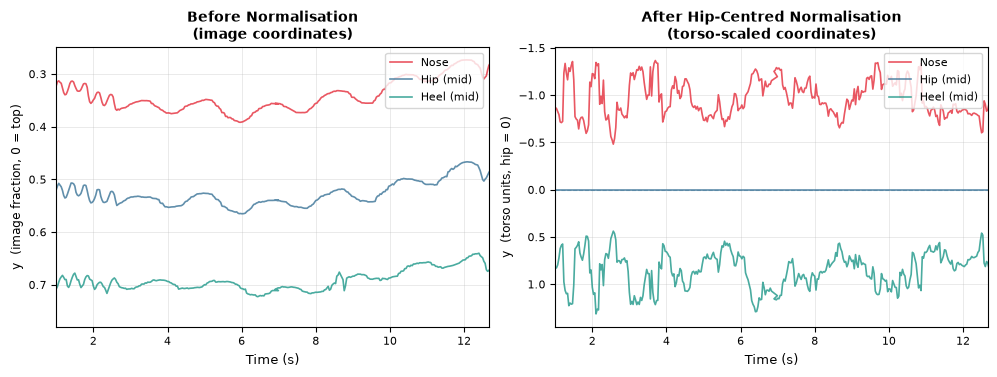
\includegraphics[width=\textwidth]{figures_new/fig34_landmark_normalization}
\caption{Landmark vertical coordinates before (left) and after (right)
hip-centred normalisation for an example video. Before normalisation, the
trajectories drift with the runner's absolute position in the frame. After
normalisation, all trajectories oscillate stably about zero (the hip
reference) with consistent amplitude regardless of camera distance or
runner position.}
\label{fig:landmark_normalization}
\end{figure}

% ---------------------------------------------------------------------
\section{Motion Signal Extraction}
\label{sec:method-signals}

From the filtered, normalised landmarks, a set of one-dimensional \emph{motion
signals} is derived for cycle detection. Each signal is a scalar time series
whose periodic structure reflects the running cycle.
Table~\ref{tab:signals} lists the candidate signals.

\begin{table}[htbp]
\centering
\caption{Candidate one-dimensional motion signals used for running-cycle
detection.}
\label{tab:signals}
\renewcommand{\arraystretch}{1.2}
\begin{tabularx}{\textwidth}{l X}
\toprule
Signal & Definition (per frame) \\
\midrule
head-Y & Vertical position of the head/nose landmark \\
hip-Y & Vertical position of the hip (pelvis) landmark \\
heel-Y & Vertical position of the heel landmark \\
toe-Y & Vertical position of the toe (foot index) landmark \\
\texttt{contact\_diff} & Foot-contact proxy from the heel/toe landmarks (left--right contact difference) \\
\texttt{AP\_diff} & Anterior--posterior (horizontal) displacement difference between feet \\
\texttt{V\_diff} & Vertical displacement difference between feet \\
\bottomrule
\end{tabularx}
\end{table}

The vertical-oscillation signals (head-Y, hip-Y) are smooth and easy to detect
but only indirectly related to foot strike, whereas the foot-derived signals
(\texttt{contact\_diff}, \texttt{AP\_diff}, \texttt{V\_diff}, heel-Y, toe-Y) are
more directly tied to ground contact but noisier
(Chapter~\ref{ch:literature-review}). The pipeline supports any single signal as
the detection driver; the comparison of signals is treated as an ablation
(Chapter~\ref{ch:results}). Each signal is smoothed and detrended before
detection to stabilise period estimation. Figure~\ref{fig:motion_signals} shows
the four main signals over an example running clip.

\begin{figure}[htbp]
\centering
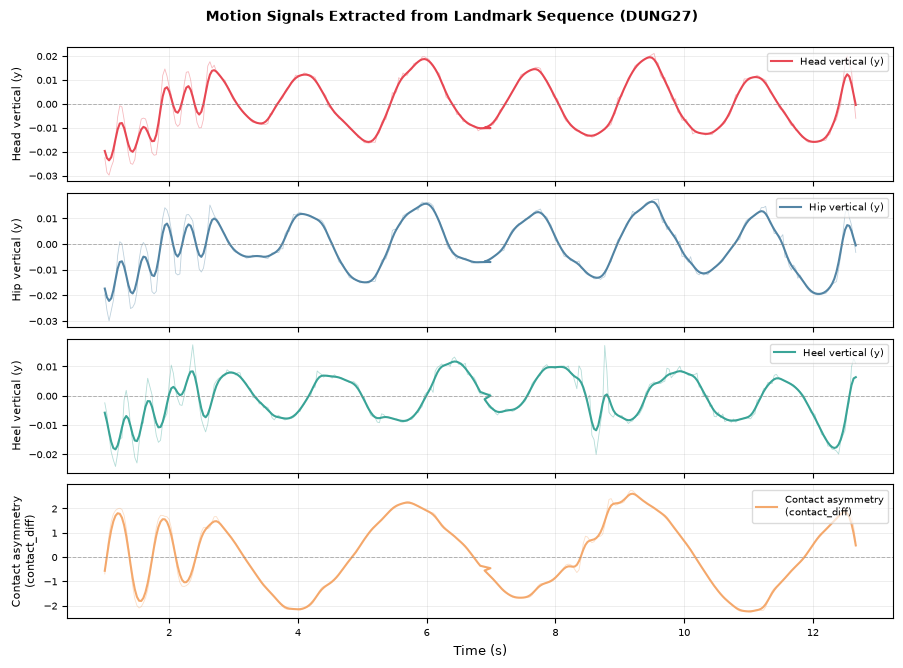
\includegraphics[width=\textwidth]{figures_new/fig35_motion_signals}
\caption{Motion signals extracted from a single running video (DUNG27). Faint
lines show the raw detrended signal; solid lines show the Gaussian-smoothed
version ($\sigma=2$). The periodic oscillation visible in all four signals
reflects the running cycle; \texttt{contact\_diff} captures left--right
foot-contact asymmetry and is used as the primary cycle-detection driver.}
\label{fig:motion_signals}
\end{figure}

% ---------------------------------------------------------------------
\section{Running Cycle Detection}
\label{sec:method-cycle}

A running cycle is bounded by successive foot-strike events of the same foot
(foot-strike-to-foot-strike, FS-to-FS). The framework provides three
interchangeable detectors --- a manual handmade segmentation, an automatic
autocorrelation-based detector, and a learned boundary detector --- followed by a
common quality-filtering step.

\subsection{Handmade Cycle Segmentation}
\label{sec:method-handmade}

In the handmade pipeline, cycle boundaries are determined manually so that each
extracted cycle is correctly segmented. This pipeline is used as an
\emph{upper bound}: it characterises how well the representation and classifier
can separate correct from false technique \emph{when segmentation is reliable},
and thereby separates the difficulty of classification from the difficulty of
automatic detection. It is not a deployable baseline, since a fielded system
cannot rely on manual segmentation.

\subsection{Autocorrelation-Based Automatic Cycle Detection}
\label{sec:method-autocorr}

The automatic baseline detects cycles without manual input. A chosen motion
signal is smoothed and detrended; its dominant period is estimated by
\emph{autocorrelation}; candidate foot-strike boundaries are located by
peak/valley detection on the signal; and the estimated period is used to
validate boundary spacing, including a correction for spurious double-stride
detections (a two-stride fix). Candidate cycles are then passed to quality
filtering. Algorithm~\ref{alg:autocorr_cycle_detection} summarises the procedure.

\begin{algorithm}[htbp]
\caption{Autocorrelation-based running cycle detection}
\label{alg:autocorr_cycle_detection}
\begin{algorithmic}[1]
\Require Filtered landmark sequence, motion signal $s$, duration bounds $[\tau_{\min}, \tau_{\max}]$
\Ensure Set of accepted FS-to-FS running cycles $C$
\State $x \gets \textsc{ExtractSignal}(s)$
\State $x \gets \textsc{Smooth}(x)$
\State $\hat{p} \gets \textsc{EstimatePeriod}(\textsc{Autocorrelation}(x))$
\State $P \gets \textsc{FindCandidateBoundaries}(x)$
\State $P \gets \textsc{TwoStrideFix}(P, \hat{p})$
\State $C \gets \emptyset$
\For{each consecutive boundary pair $(f_i, f_{i+1})$ in $P$}
    \State $\tau \gets \textsc{Duration}(f_i, f_{i+1})$
    \If{$\tau_{\min} \leq \tau \leq \tau_{\max}$ and visibility is adequate}
        \State $C \gets C \cup \{(f_i, f_{i+1})\}$
    \EndIf
\EndFor
\State \Return $\textsc{QualityFilter}(C)$
\end{algorithmic}
\end{algorithm}

This detector is the main \emph{automatic baseline} of the thesis: it uses only
information available from the video itself, with no fixed-margin assumption on
boundary placement, and produces cycles directly comparable to the handmade
ones because the downstream stages are identical.
Figure~\ref{fig:cycle_boundaries} shows an example detection result.

\begin{figure}[htbp]
\centering
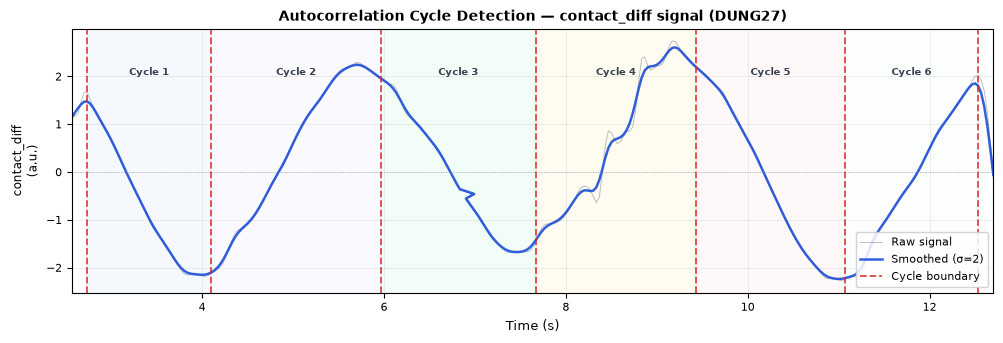
\includegraphics[width=\textwidth]{figures_new/fig36_cycle_boundaries}
\caption{Running cycle boundaries detected by the autocorrelation-based
detector overlaid on the \texttt{contact\_diff} signal for an example video
(DUNG27). Alternating shaded bands correspond to individual FS-to-FS cycles;
red dashed lines mark the detected boundaries. The periodic structure of the
signal makes the boundaries reliably locatable by the autocorrelation
procedure.}
\label{fig:cycle_boundaries}
\end{figure}

\subsection{Boundary Detector-Based Cycle Detection}
\label{sec:method-bd}

As a learned alternative to rule-based detection, a \emph{boundary detector}
(BD) replaces autocorrelation with a trained sequence model
\cite{zhang2025heelstrike, sui2020gaitsegmentation}. The BD is a BiLSTM that
consumes a sliding window of frames and predicts the probability that the
central frame is a foot-strike boundary; ground-truth boundaries are taken from
the endpoints of handmade single-cycle clips. At inference, the per-frame
boundary probabilities are smoothed and thresholded, peaks are taken as
boundaries, and consecutive boundaries define FS-to-FS cycles, which are then
quality-filtered exactly as for the autocorrelation detector. The BD is treated
as a supplementary pipeline.

\subsection{Cycle Quality Filtering}
\label{sec:method-quality}

Regardless of detector, candidate cycles pass through a common
\emph{quality-filtering} step before being accepted. Cycles whose duration falls
outside the plausible running-cycle range, whose constituent landmarks have
insufficient visibility, or which cannot be sampled into the required number of
phases are rejected. This step enforces a consistent definition of a usable
cycle across all pipelines, so that the only intended difference between them is
how boundaries are obtained. The rejected-cycle statistics are later used to
analyse where the automatic pipeline loses data (Chapter~\ref{ch:results}).

% ---------------------------------------------------------------------
\section{Eight-Phase Cycle Sampling}
\label{sec:method-phases}

Each accepted cycle is resampled into a fixed number of \emph{gait phases} so
that cycles of different absolute durations become directly comparable. Eight
phases are used, spanning one full FS-to-FS cycle:

\begin{figure}[htbp]
    \centering
    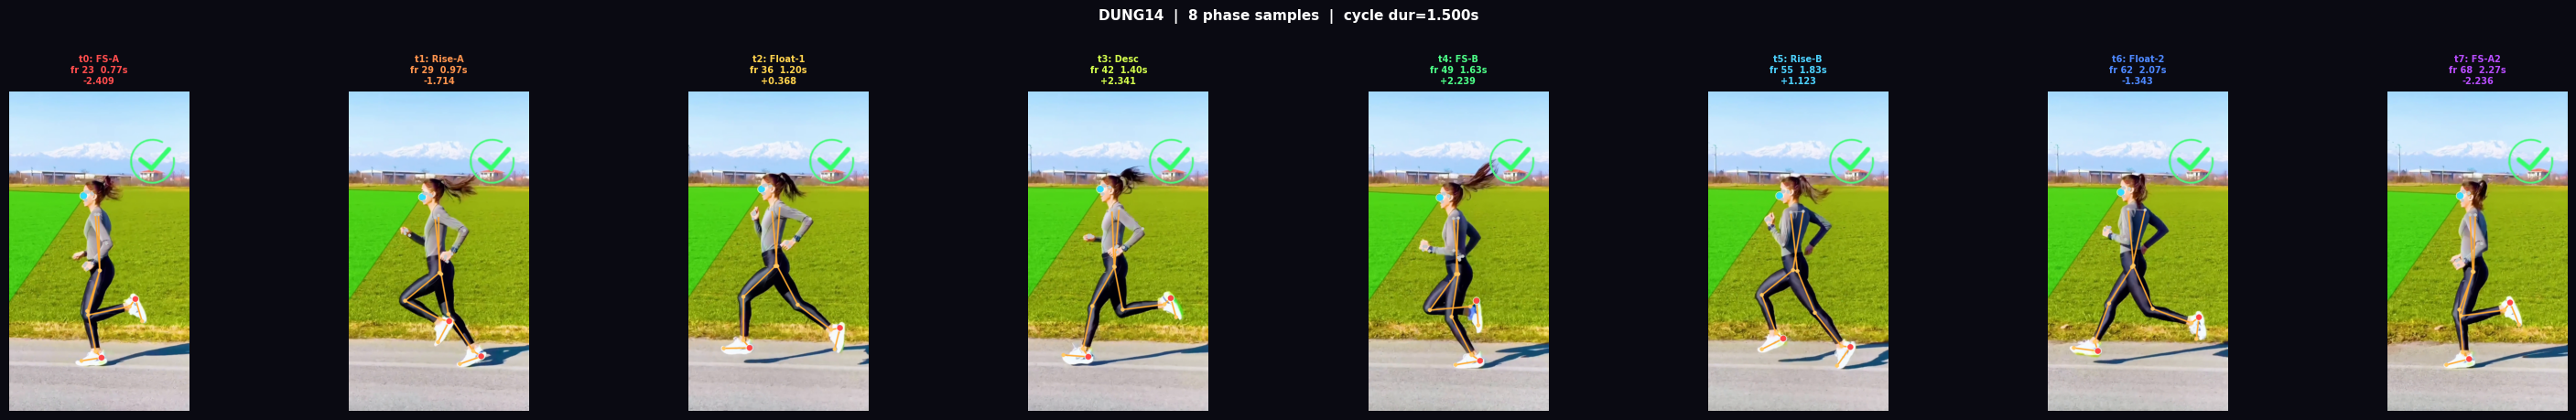
\includegraphics[width=\textwidth]{figures/8_sample_phase.png}
    \caption{Example of eight-phase sampling from an automatically detected running cycle.}
    \label{fig:8phase_sampling}
\end{figure}

Sampling at fixed phases (rather than fixed frame offsets) normalises for
cadence, so that "the same phase" denotes the same point in the running cycle
across runners and speeds \cite{inostroza2025runningcycle}. The eight-phase
sampling defines the temporal length of every representation that follows; its
sufficiency relative to finer samplings is examined as a frames-per-cycle
ablation in Chapter~\ref{ch:results}.

% ---------------------------------------------------------------------
\section{Landmark-Based Pose Representation}
\label{sec:method-landmark-rep}

In the landmark representation, each of the eight phases is encoded by the
normalised coordinates of the selected landmarks, optionally augmented with
\emph{velocity} (the inter-phase change in coordinates) and other derived
quantities. The result is a compact, fixed-size sequence per cycle that is
invariant to appearance by construction. This representation is the basis of the
main automatic baseline and of the model, feature, and signal ablations.

% ---------------------------------------------------------------------
\section{Image-Based Cycle Representation}
\label{sec:method-image-rep}

In the image representation, each phase is encoded as an RGB \emph{crop} centred
on the runner. A stable bounding box is computed per cycle from the pose
estimates (for example a median box over the cycle) and used to crop and resize
each sampled frame to a fixed resolution, yielding an eight-frame image sequence
per cycle. This representation retains appearance information absent from
landmarks --- silhouette, limb contour, clothing-relative motion --- at the cost
of higher dimensionality and sensitivity to crop stability. To ensure a
\emph{fair} comparison, the image pipeline uses exactly the same automatic cycle
source as the landmark baseline, so that the two differ only in representation
(Chapter~\ref{ch:results}).

% ---------------------------------------------------------------------
\section{Classification Models}
\label{sec:method-models}

Several classifiers are used across the representations and pipelines, chosen to
span a range of temporal modelling capacity.
Figure~\ref{fig:model_architectures} shows the layer-by-layer architectures of
the four landmark-based models.

\begin{figure}[htbp]
\centering
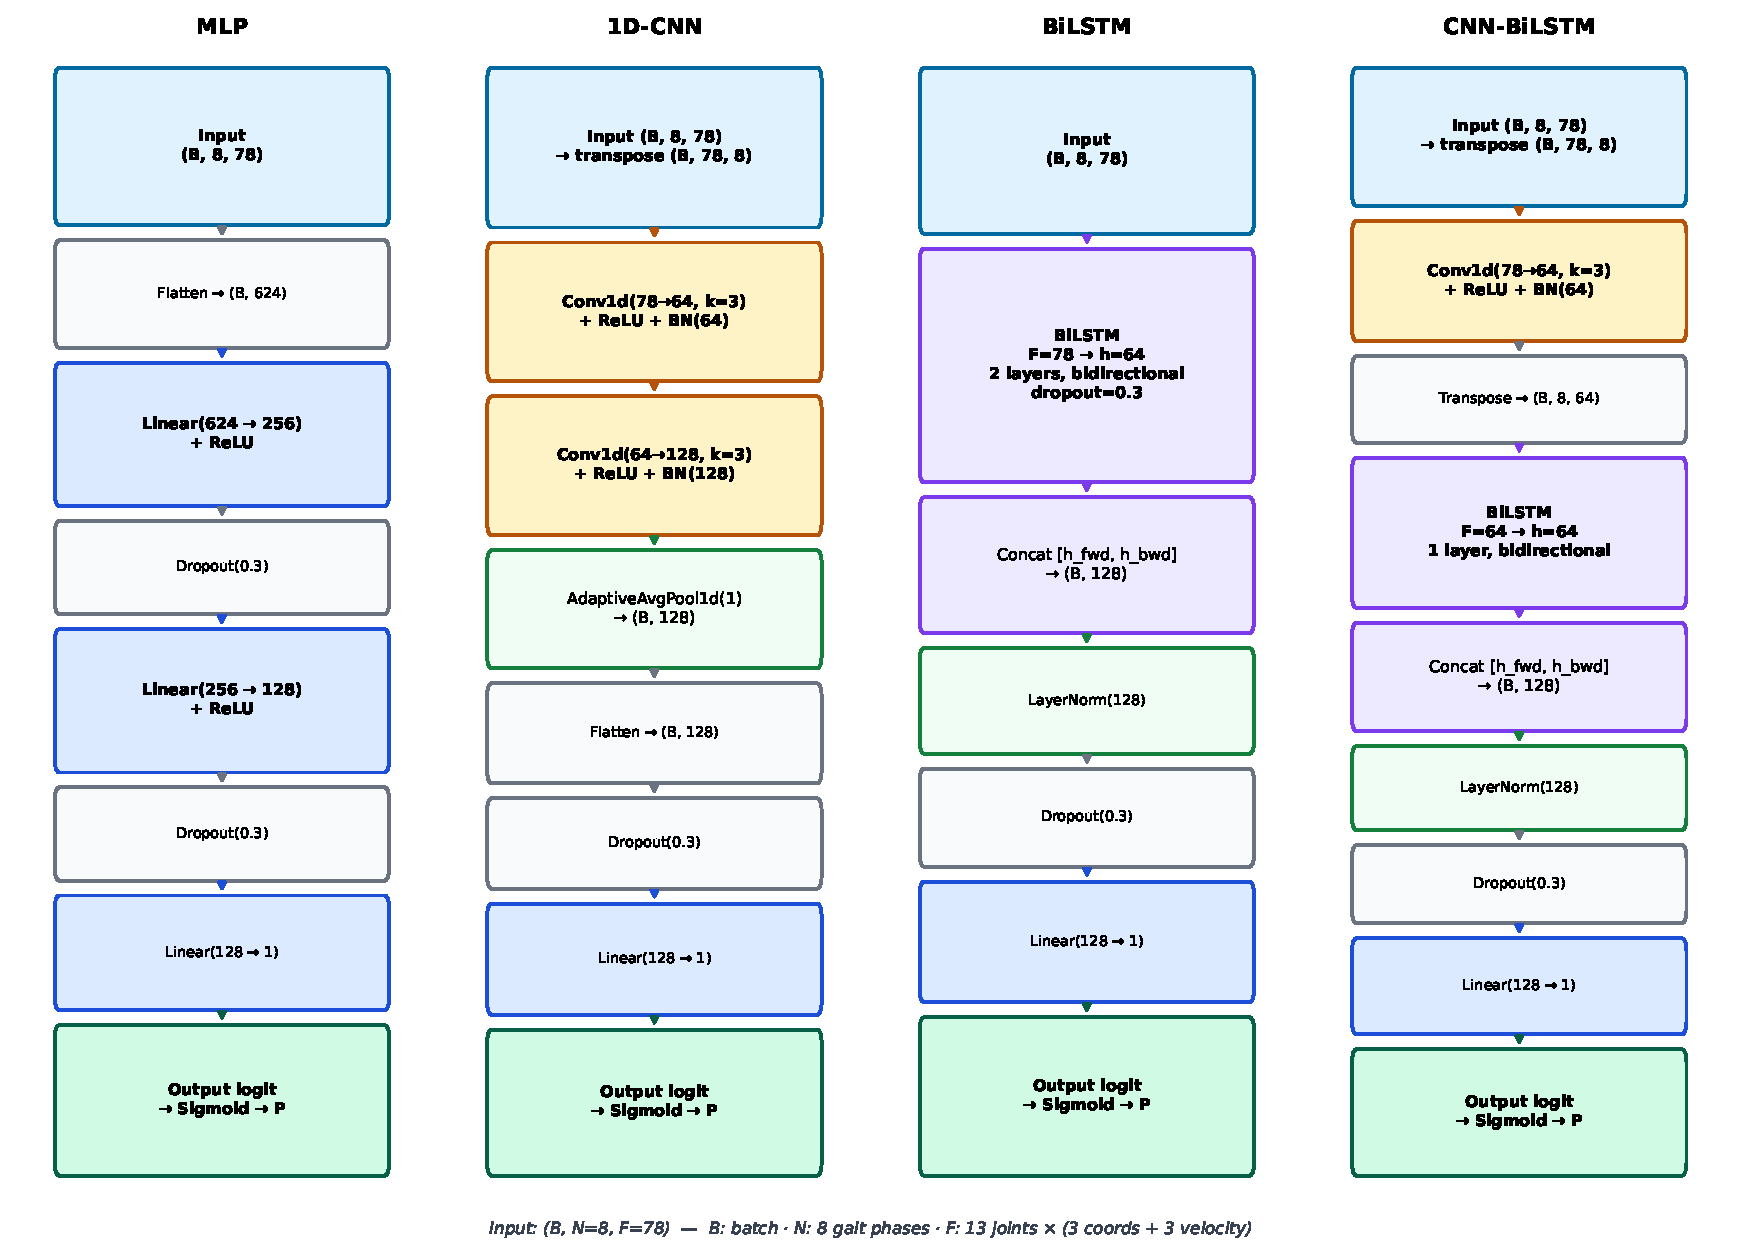
\includegraphics[width=\textwidth]{figures_new/fig_model_architectures}
\caption{Layer-by-layer architectures of the four landmark-based classifiers.
All models receive an input tensor of shape $(B,\,8,\,78)$ --- batch size,
eight gait phases, and $F{=}78$ features (13 joints $\times$ 3 coordinates
$+$ 3 velocity components) --- and produce a single binary logit. Colour
indicates layer type: blue --- linear; amber --- convolutional; violet ---
recurrent (BiLSTM); green --- normalisation or pooling; grey --- utility
(flatten, dropout).}
\label{fig:model_architectures}
\end{figure}

\subsection{MLP Baseline}
\label{sec:method-mlp}

The multilayer perceptron flattens the eight-phase landmark sequence into a
single vector and learns a static mapping to the correct/false decision. It does
not model temporal order, but is fast and low-variance, which can be
advantageous for short, well-aligned inputs.

\subsection{One-Dimensional CNN}
\label{sec:method-cnn}

The 1D-CNN applies temporal convolutions across the eight-phase sequence,
capturing local kinematic patterns with relatively few parameters before a
classification head \cite{ordonez2016deephar}.

\subsection{BiLSTM}
\label{sec:method-bilstm}

The bidirectional LSTM processes the phase sequence in both directions, so that
each phase is represented in the context of the entire cycle, capturing
longer-range temporal dependencies than the convolutional model
\cite{hochreiter1997lstm, schuster1997bidirectional}.

\subsection{CNN-BiLSTM}
\label{sec:method-cnn-bilstm}

The CNN-BiLSTM hybrid first extracts local features with one-dimensional
convolutions and then models their temporal evolution with a BiLSTM, combining
local pattern extraction with sequence modelling \cite{donahue2015lrcn}.

\subsection{MobileNetV2-LSTM}
\label{sec:method-mobilenet}

For the image representation, a MobileNetV2--LSTM model is used: a MobileNetV2
convolutional backbone encodes each RGB crop into a feature vector, and an LSTM
aggregates the eight per-phase feature vectors into a cycle-level prediction. The
backbone may be frozen or partially fine-tuned
\cite{sandler2018mobilenetv2, donahue2015lrcn}. This model operates on image
crops rather than landmark coordinates and is therefore used only in the
image-based pipeline.

\subsection{GRU for Raw Sequence Modeling}
\label{sec:method-gru}

To probe whether explicit cycle cutting is necessary, a recurrent model
(a gated recurrent unit, GRU, alongside a BiLSTM) is applied to the
\emph{raw} pose sequence of an entire video, without segmentation into cycles.
Here one sample corresponds to one video, so this is an exploratory,
supplementary configuration rather than part of the cycle-based comparison.

% ---------------------------------------------------------------------
\section{Cycle-Level and Video-Level Prediction}
\label{sec:method-cycle-video}

Because each video yields several cycles, predictions are produced at two
levels. \emph{Cycle-level} prediction treats each detected cycle as an
independent sample. \emph{Video-level} prediction aggregates a video's cycle
predictions into a single decision; three aggregation rules are considered:
\emph{majority vote}, \emph{mean probability}, and \emph{confidence-weighted
vote}. Since the underlying data unit is the video, video-level prediction is
the more faithful measure of practical performance; both levels are reported so
that the effect of aggregation can be examined (Chapter~\ref{ch:results}).

% ---------------------------------------------------------------------
\section{Threshold Selection}
\label{sec:method-threshold}

Each probabilistic classifier requires a \emph{decision threshold} to convert
predicted probabilities into a correct/false label. Two settings are
considered: the default threshold of $0.5$, and a \emph{tuned} threshold
selected on the \emph{validation} set by sweeping candidate thresholds and
choosing the one that maximises validation macro-F1, which is then applied
unchanged to the test set. Selecting the threshold on validation rather than on
test avoids optimistic bias; reporting both the default and the tuned result
makes any threshold overfitting visible. Every reported metric states which
threshold setting it uses.

% ---------------------------------------------------------------------
\section{Implementation Outputs}
\label{sec:method-outputs}

The pipeline is implemented as a sequence of self-contained, configurable
notebooks, each writing standardised outputs --- per-cycle and per-video
prediction files, result summaries, cycle-detection statistics, and diagnostic
figures --- to a fixed directory structure. These artefacts provide the inputs
to the controlled comparisons, ablations, and quality analyses presented in
Chapter~\ref{ch:results}, and are designed so that missing files degrade
gracefully rather than invalidating downstream aggregation.

% End of Chapter 3